% !TeX program = xelatex
% 应用随机过程 笔记（LaTeX 版）
% 依据手写笔记整理：第〇章 引言、第一章 马氏链（第 2、3 章跳过程与布朗运动待补）。
\documentclass[11pt]{ctexart}
\usepackage[a4paper,margin=2.3cm]{geometry}
\usepackage{amsmath,amssymb,amsthm,mathtools}
\usepackage{booktabs}
\usepackage{array}
\usepackage{tikz}
\usetikzlibrary{arrows.meta,positioning,calc,decorations.pathmorphing,decorations.pathreplacing}
\usepackage[colorlinks=true,linkcolor=blue!55!black,urlcolor=blue!55!black]{hyperref}

\setcounter{secnumdepth}{-2}
\setcounter{tocdepth}{1}

\theoremstyle{definition}
\newtheorem*{definition}{定义}
\newtheorem*{proposition}{命题}
\newtheorem*{theorem}{定理}
\newtheorem*{lemma}{引理}
\newtheorem*{corollary}{推论}
\newtheorem*{example}{例}
\newtheorem*{remark}{注}
\newtheorem*{question}{问}
\theoremstyle{remark}

\newcommand{\R}{\mathbb{R}}
\newcommand{\Z}{\mathbb{Z}}
\newcommand{\N}{\mathbb{N}}
\newcommand{\E}{\mathbb{E}}
\newcommand{\Pp}{\mathbb{P}}
\newcommand{\ind}[1]{\mathbf{1}_{\{#1\}}}
\newcommand{\darr}{\;\Rightarrow\;}
\newcommand{\reach}{\to}
\newcommand{\comm}{\leftrightarrow}

% 章标题（手工编号，与小节编号 0.x / 1.x 对应）
\newcommand{\chap}[1]{%
  \clearpage
  \vspace*{0.5em}
  {\centering\LARGE\bfseries #1\par}
  \vspace{0.4em}
  \addcontentsline{toc}{section}{#1}}
\newcommand{\secn}[2]{\subsection*{#1\quad #2}\addcontentsline{toc}{section}{#1\quad #2}\markboth{#1\quad #2}{}}

\title{\heiti 应用随机过程\\[0.3em]\large 课堂笔记（LaTeX 整理版）}
\author{}
\date{2026 年 10 月}

\begin{document}
\maketitle
\vspace{-3em}

\begin{abstract}
\noindent
本笔记整理自《应用随机过程》课堂手写笔记，目前包含第〇章（引言）与第一章（马氏链）的完整内容；
按原计划还有第二章（跳过程）与第三章（布朗运动），待后续补充。记号约定：$\Pp_\mu$ 表示初分布为
$\mu$ 时的概率律，$\E_i$ 表示 $X_0=i$ 时的期望；$\tau_i=\inf\{n\ge 0:X_n=i\}$ 为首达时，
$\sigma_i=\inf\{n\ge 1:X_n=i\}$ 为首入时；$V_i=\sum_{n\ge0}\ind{X_n=i}$ 为访问总次数。
\end{abstract}

\tableofcontents

%======================================================================
\chap{第〇章\quad 引言}

\secn{0.1}{课程地图（MAP）}

本课程在整个概率课程体系中的位置大致如下：

\begin{itemize}
  \item \textbf{概率论}：独立随机变量（R.V.）的极限定理，是整个体系的出发点；
  \item \textbf{应用随机过程}（本课程）：相依随机变量序列的极限，由概率论发展而来；
  \item \textbf{高维概率论}：非极限定理、精细不等式；
  \item \textbf{高等概率论}：独立情形的复杂极限（旁注：突变、测度论）；
  \item \textbf{应用随机分析}：布朗运动、随机微积分，由应用随机过程发展而来；
  \item \textbf{随机过程论}：由高等概率论发展而来；
  \item \textbf{随机分析}：其基础工具之一是泛函分析。
\end{itemize}

按“时间参数集 $I$”与“状态空间 $S$”的离散/连续分类，随机过程 $\{X_t\}_{t\in I}$ 可分为四类，
本课程的三个主体章节各占一格：

\begin{center}
\begin{tabular}{c|cc}
\toprule
 $\{X_t\}_{t\in I}$ & 离散状态 & 连续状态 \\
\midrule
 离散时间 & 第一章\quad 马氏链 & --- \\
 连续时间 & 第二章\quad 跳过程 & 第三章\quad 布朗运动 \\
\bottomrule
\end{tabular}
\end{center}

\secn{0.2}{模型与研究方法简史}

\textbf{20 世纪前半叶}：独立 R.V. 的和（极限定理）、严格 M.B.、布朗运动。

\textbf{20 世纪后半叶至今}：模型与研究方法可概括为下表。

\begin{center}
\begin{tabular}{c|p{5.6cm}|p{6.4cm}}
\toprule
 & 离散（组合、优化、图论） & 连续（泛函、PDE、微分流形） \\
\midrule
一般理论
 & 半群 / 生成元（1940--50s）；伊辛、渗流（1950--70s）；相互作用粒子系统（1970--80s）
 & 鞅问题（1970--80s）；随机积分（1940--50s）及其推广（1960--80s）；随机 PDE（非奇异）（1980--90s） \\
\midrule
具体问题
 & 标度极限、可解模型、集中不等式、轨道性质、随机环境；\par
 量子 / 统计物理：相变、随机曲面、SLE、CLE、随机量子化、随机 Yang--Mills、自旋玻璃；\par
 几何 / 代数：随机矩阵、随机几何、流形与群上的随机性；\par
 生物 / 化学：聚合物、分支过程；\par
 统计 / 计算：随机图论、收敛算法
 & 奇异 SPDE、热核估计、随机动力系统、流体力学极限、大偏差、噪声退化 \\
\bottomrule
\end{tabular}
\end{center}

\secn{0.3}{预备知识：极限定理回顾}

设 $\{X_n\}$ 为随机变量序列，记 $A_n:=\{|X_n-X|>\varepsilon\}$，则以下几条是全课程反复使用的工具：
\begin{itemize}
  \item 依概率收敛：$X_n\xrightarrow{\ P\ }X\iff \Pp(A_n)\to 0$；
  \item 几乎必然收敛：$X_n\xrightarrow{\ \mathrm{a.s.}\ }X\iff \Pp\Bigl(\bigcup_{n\ge N}A_n\Bigr)\to 0\ (N\to\infty)$；
  \item Borel--Cantelli 引理：$\sum_{n\ge1}\Pp(A_n)<+\infty\ \darr\ \Pp\Bigl(\bigcup_{n\ge N}A_n\Bigr)\to 0$；
  \item 有界收敛定理：$X_n\xrightarrow{\ P\ }X$，$|X_n|\le M$ a.s.\ $\darr\ \E|X_n-X|\to 0$；
  \item 单调收敛定理：$X_n\ge 0$，$X_n\uparrow X\ \darr\ \E X_n\to\E X$；
  \item Lebesgue 控制收敛定理：$X_n\xrightarrow{\ \mathrm{a.s.}\ }X$，$|X_n|<Y$，$\E Y<+\infty\ \darr\ \E X_n\to\E X$；
  \item Fubini 定理（Tonelli）：$X_t\ge0$ 或 $\int_0^{+\infty}\E|X_t|\,dt<+\infty$，则
  \[
    \E\int_0^{+\infty}X_t\,dt=\int_0^{+\infty}\E X_t\,dt.
  \]
\end{itemize}

\secn{0.4}{随机元}

设 $(\Omega,\mathcal{F},\Pp)$ 为概率空间，$S$ 为可测空间。取值于 $S$ 的随机变量称为
\textbf{随机元}：$X_n,\,X_t:(\Omega,\mathcal{F},\Pp)\to S$。于是

\[
\{X_n:n\ge0\}:(\Omega^{\Z^+},\mathcal{F}^{\Z^+},\Pp)\to S^{\Z^+},
\qquad
\{X_t:t\ge0\}:(\Omega^{\R^+},\mathcal{F}^{\R^+},\Pp)\to S^{\R^+},
\]

即一个随机过程（序列）可以看作乘积空间上的一个随机元。

%======================================================================
\chap{第一章\quad 马氏链}

\secn{1.1}{定义与例子}

设 $\{X_n:n\ge0\}$ 的状态空间 $S$ 离散。

\begin{definition}[马氏链]
若对 $\forall n\ge0$ 及任意 $i_0,i_1,\dots,i_{n-1},\,i,\,j\in S$，存在 $p_{ij}$ 使得
\[
\Pp\bigl(X_{n+1}=j \mid X_n=i,\ X_{n-1}=i_{n-1},\ \dots,\ X_0=i_0\bigr)=p_{ij},
\]
则称 $\{X_n:n\ge0\}$ 为（时齐）\textbf{马氏链}，$p_{ij}$ 称为转移概率。
\end{definition}

\begin{proposition}
转移概率满足：（1）$p_{ij}\ge0$，$\sum_j p_{ij}=1$；（2）$p_{ij}=\Pp(X_{n+1}=j\mid X_n=i)$。

证明：（2）由全概率公式对历史求和即得。
\end{proposition}

\begin{example}[一维简单随机游动，SRW]
$S=\Z$，$p_{i,i-1}=p_{i,i+1}=\tfrac12$。等价地：取 $\xi_1,\xi_2,\dots$ i.i.d.，
$\Pp(\xi_n=1)=\Pp(\xi_n=-1)=\tfrac12$；令 $S_0:=0$（或与 $\{\xi_n\}$ 独立），
\[
S_n:=S_0+\xi_1+\dots+\xi_n=S_{n-1}+\xi_n ,
\]
其中 $\xi_n$ 称为\textbf{步长}。
\end{example}

\begin{example}[$d$ 维 SRW]
设 $e_i$（$i=1,\dots,d$）为坐标单位向量，
$\Pp(\xi=e_i)=\Pp(\xi=-e_i)=\tfrac{1}{2d}$。在边界上可加约束：
\begin{itemize}
  \item \textbf{吸收壁} $x^*$：$p_{(x^*,y),(x^*,y)}=1$；
  \item \textbf{反射壁} $x^*$：$p_{(x^*,y),(x^*-1,y)}=1$，
\end{itemize}
其中 $(x^*,y)$ 为边界上的状态。
\end{example}

\begin{example}[两状态马氏链]
参数 $p_{01},p_{10}$，转移图如下：
\[
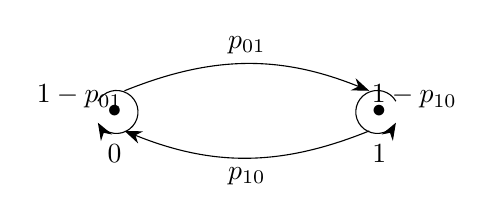
\begin{tikzpicture}[scale=1.05,>={Stealth[length=2.2mm]}]
  \node (A) at (0,0) {$\bullet$};
  \node[below=1mm] at (A.south) {$0$};
  \node (B) at (3.2,0) {$\bullet$};
  \node[below=1mm] at (B.south) {$1$};
  \draw[->] ($(A.north)+(0.12,0.05)$) to[bend left=22] node[above]{$p_{01}$} ($(B.north)+(-0.12,0.05)$);
  \draw[->] ($(B.south)+(-0.12,-0.05)$) to[bend left=22] node[below]{$p_{10}$} ($(A.south)+(0.12,-0.05)$);
  \draw[->] (A.150) arc[start angle=150,end angle=-150,radius=2.6mm] node[pos=0.35,left]{$1-p_{01}$};
  \draw[->] (B.30) arc[start angle=30,end angle=330,radius=2.6mm] node[pos=0.35,right]{$1-p_{10}$};
\end{tikzpicture}
\]
\end{example}

\begin{example}[Ehrenfest 模型]
共 $N$ 个球分装在箱 $A,B$ 中；$X_n:=$ 第 $n$ 次操作后 $A$ 中的球数，$S=\{0,1,\dots,N\}$。
每次等可能地取出一个球放入另一箱，故从状态 $i$ 出发：
$i\to i-1$ 的概率为 $\tfrac{i}{N}$（从 $A$ 中取球），$i\to i+1$ 的概率为 $1-\tfrac{i}{N}$。
\[
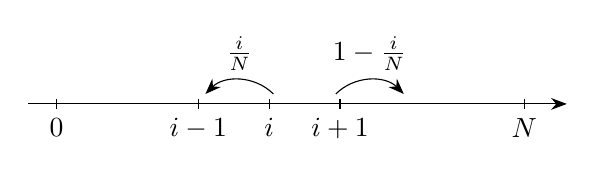
\begin{tikzpicture}[scale=0.9,>={Stealth[length=2mm]}]
  \draw[->] (-0.4,0)--(7.2,0);
  \foreach \x/\l in {0/0,2/i-1,3/i,4/i+1,6.6/N}{
    \draw (\x,0.07)--(\x,-0.07) node[below]{$\l$};}
  \draw[->] (3.06,0.14) to[bend right=45] node[above]{$\frac{i}{N}$} (2.1,0.14);
  \draw[->] (3.94,0.14) to[bend left=45] node[above]{$1-\frac{i}{N}$} (4.9,0.14);
\end{tikzpicture}
\]
\end{example}

\begin{example}[更新过程]
设 $L_1,L_2,\dots\ \doteq\ L$ i.i.d.，$L_n$ 为第 $n$ 个物品的寿命。令
$S_0=0$，$S_n:=L_1+\dots+L_n$（$n\ge1$）为\textbf{更新时刻}，
\[
N_n:=\max\{k:S_k\le n\}
\]
为到时刻 $n$ 的更新次数。\textbf{$\{N_n\}$ 不是马氏链}。

定义\textbf{余寿} $X_n:=S_{r_n}-n$，其中 $r_n:=\inf\{r:S_r\ge n\}$。则 $\{X_n\}$ 是马氏链：
$S=\Z^+$，且
\[
p_{0,i}=\Pp(L=i+1)\quad(\forall i\ge0),\qquad p_{i,i-1}=1\quad(\forall i\ge1).
\]
\end{example}

\begin{example}[图上的随机游动]
设 $G=(V,E)$，顶点 $i\mapsto d_i$（度）。取 $S=V$，
\[
p_{ij}=
\begin{cases}
\dfrac{1}{d_i}, & j\sim i,\\[0.4em]
0, & j\nsim i.
\end{cases}
\]
\end{example}

\paragraph{马氏性}
设 $\{X_n:n\ge0\}$ 为马氏链，$X_0\sim\mu$，则
\begin{align*}
\Pp(X_0=i_0,X_1=i_1,\dots,X_n=i_n)
&=\Pp(X_0=i_0,\dots,X_{n-1}=i_{n-1})\cdot\Pp(X_n=i_n\mid \ast)\\
&=\Pp(\ast)\cdot p_{i_{n-1}i_n}
=\dots=\mu_{i_0}\,p_{i_0i_1}\cdots p_{i_{n-1}i_n}.
\end{align*}

\begin{proposition}[马氏性]
设 $\{X_n:n\ge0\}$ 为马氏链。令 $Y_m:=X_{n+m}$（$m\ge0$，$n\ge1$），则 $\{Y_m\}$ 在
$\{X_n=i\}$ 条件下是从 $i$ 出发、转移矩阵为 $P$ 的马氏链，且与 $\{X_0,X_1,\dots,X_{n-1}\}$ 独立。
\end{proposition}

\begin{proof}
记 $A:=\{X_n=i\}$，$B:=\{\vec{Y}=\vec{j}\}$，$C:=\{\vec{Z}=\vec{z}\}$，其中
$\vec{Y}:=(Y_0,\dots,Y_m)$，$\vec{j}:=(j_0,\dots,j_m)$，$\vec{Z}:=(X_0,\dots,X_{n-1})$，
$\vec{z}:=(z_0,\dots,z_{n-1})$。则只需证：
\[
(1)\ \Pp_A(B)=\ind{j_0=i}\,p_{j_0j_1}\,p_{j_1j_2}\cdots p_{j_{m-1}j_m};
\qquad
(2)\ \Pp_A(BC)=\Pp_A(B)\cdot\Pp_A(C).
\]
由 $\{X_n\}$ 为马氏链可知
\[
\Pp(ABC)=\mu_{z_0}\,p_{z_0z_1}\cdots p_{z_{n-2}z_{n-1}}\;p_{z_{n-1}i}\;
\ind{j_0=i}\,p_{j_0j_1}\cdots p_{j_{m-1}j_m},
\]
对上式关于 $\vec{z}$ 的各分量求和即可验证 (1)(2)。
\end{proof}

\begin{definition}[$n$ 步转移概率]
\[
p_{ij}^{(n)}:=\Pp(X_n=j\mid X_0=i)
=\sum_{i_1,\dots,i_{n-1}}\Pp(X_1=i_1,\dots,X_{n-1}=i_{n-1},X_n=j)
=\bigl(P^n\bigr)_{ij}.
\]
\end{definition}

\begin{proposition}[C--K 方程]
$P^{\,n+m}=P^{\,n}P^{\,m}$。
\end{proposition}

\begin{proof}
\begin{align*}
\Pp(X_{n+m}=j\mid X_0=i)
&=\sum_k\Pp(X_{n+m}=j,\,X_m=k\mid X_0=i)\\
&=\sum_k\Pp(X_m=k\mid X_0=i)\cdot\Pp(X_{n+m}=j\mid X_m=k,X_0=i)\\
&\xrightarrow{\ \text{马氏性}\ }
\sum_k\bigl(P^m\bigr)_{ik}\bigl(P^n\bigr)_{kj}=:\bigl(P^{m+n}\bigr)_{ij}. \qedhere
\end{align*}
\end{proof}

\secn{1.2}{不变分布与可逆分布}

\subsection*{1.2.1\quad 不变分布}

记 $\Pp_\mu,\Pp_i$，其中 $\Pp_i(A)=\Pp_\mu(A\mid X_0=i)$，且
\[
\Pp_\mu(A)=\sum_i\mu_i\,\Pp_i(A),\qquad \mu\ \text{为概率行向量}.
\]
于是 $\Pp_\mu(X_1=j)=\sum_i\mu_i p_{ij}=(\mu P)_j$；$X_n\mid X_0\sim\mu$ 的分布为 $\mu P^n$。

\begin{definition}[不变测度 / 不变分布]
$\pi=(\pi_j)_{j\in S}$ 称为 $(S,P)$ 上的\textbf{不变测度}，若其满足 $\pi P=\pi$；
当 $\pi$ 还是概率分布时称为\textbf{不变分布}。
\end{definition}

此时若 $X_0\sim\pi$，则 $(X_0,X_1,\dots,X_n)\ \doteq\ (X_m,X_{m+1},\dots,X_{m+n})$，
$\forall\,n,m\ge1$，称 $\{X_n\}$ 为\textbf{平稳过程}。

\paragraph{流量角度}
平稳过程（按定义）$\iff \pi_i=\sum_j\pi_jp_{ji}$，而
\[
\iff\ \sum_{j\ne i}\pi_jp_{ji}=\pi_i-\pi_ip_{ii}=\sum_{j\ne i}\pi_ip_{ij},
\]
即“流入 $i$ 节点之流量 $=$ 流出 $i$ 节点之流量”。

\begin{example}[更新过程的不变分布]
余寿链 $X_n$：$p_{0,i}=\Pp(L=i+1)$（$i\ge0$），$p_{i,i-1}=1$（$i\ge1$）。
考虑 $A=\{i,i+1,\dots\}$ 之流量：跨过割线进入 $A$ 的流量只能来自 $0\to i$ 的跳跃，
而离开 $A$ 的流量为 $\pi_i\cdot p_{i,i-1}$，故
\[
\pi_0\cdot\Pp(L\ge i+1)=\pi_i,
\qquad
\sum_{i=0}^{+\infty}\pi_i=1 .
\]
于是 $\pi_0\bigl(1+\Pp(L\ge2)+\cdots\bigr)=1$，即 $\pi_0=\dfrac{1}{\E L}$。 \qed
\end{example}

\begin{example}
$S=\Z^+$，$p_{01}=1$；$\forall i\ge1$：$p_{i,i-1}=\dfrac{\lambda}{\lambda+1}$，
$p_{i,i+k}=\dfrac{p_k}{\lambda+1}\ (\forall k\ge1)$，其中 $\sum_k p_k=1$。求其不变分布。

考虑 $A=\{i,i+1,\dots\}$。
\begin{itemize}
  \item $i=1$：$\pi_0=\pi_1\cdot\dfrac{\lambda}{\lambda+1}$；
  \item $i\ge2$：$\pi_i\,\dfrac{\lambda}{\lambda+1}=\sum_{j=1}^{i-1}\pi_j\,\dfrac{f_{i-j}}{\lambda+1}$，
        其中 $f_r:=p_r+p_{r+1}+\cdots$。
\end{itemize}
对 $i\ge2$ 求和并换序：
\[
\frac{\lambda}{\lambda+1}\sum_{i\ge2}\pi_i
=\sum_{i\ge2}\sum_{j=1}^{i-1}\pi_j\frac{f_{i-j}}{\lambda+1}
=\sum_{j\ge1}\pi_j\sum_{i\ge j+1}\frac{f_{i-j}}{\lambda+1}
\]
\[
\darr\ \ 1-\pi_0-\pi_1=\frac{1}{\lambda}\,(1-\pi_0)\sum_{r=1}^{+\infty}f_r .
\]
记 $m:=\sum_{r=1}^{+\infty}f_r=\sum_{k=1}^{+\infty}k\,p_k$，则
$m=+\infty$ 时不变分布不存在；$m<+\infty$ 时
\[
\pi_0=\frac{\lambda-m}{2\lambda-m+1},
\qquad
\pi_1=\frac{\lambda+1}{\lambda}\,\pi_0. \qed
\]
\end{example}

\subsection*{1.2.2\quad 可逆分布}

\begin{definition}[配称测度]
$\pi=(\pi_j)_{j\in S}$ 称为 $(S,P)$ 的\textbf{配称测度（分布）}，若其满足
\[
\pi_ip_{ij}=\pi_jp_{ji}
\qquad(\mathrm{flow}_{i\to j}=\mathrm{flow}_{j\to i}).
\]
\end{definition}

易证：$\pi$ 是配称分布 $\darr$ $\pi$ 是不变分布。故配称分布亦称为\textbf{可逆分布}。

\begin{definition}[逆过程]
设 $\{X_n\}$ 为马氏链，$\pi$ 为不变分布，转移概率为 $P$。对固定 $N\ge2$，
令 $Y_n:=X_{N-n}$，则 $\{Y_n\}$ 是马氏链，转移概率为
\[
\widehat{P}_{ij}=\Pp(Y_{n+1}=j\mid Y_n=i)
=\Pp(X_{N-n-1}=j\mid X_{N-n}=i)
=\frac{\Pp(X_{N-n-1}=j,\,X_{N-n}=i)}{\Pp(X_{N-n}=i)}
=\frac{\pi_jp_{ji}}{\pi_i}.
\]
若 $\{Y_n\}\ \doteq\ \{X_n\}$，则 $\widehat{P}_{ij}=p_{ij}$，即
$\pi_ip_{ij}=\pi_jp_{ji}$，$\pi$ 为可逆分布。
\end{definition}

\begin{example}[生灭链]
$p_{i,i+1}=b_i$，$p_{i,i-1}=d_i$，$\forall i\ge0$；$b_0=1$，$b_i+d_i=1$。
\[
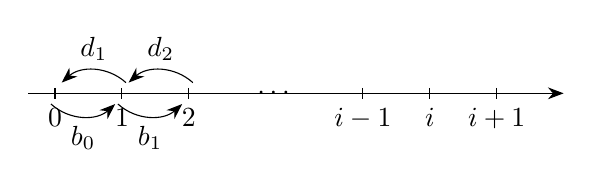
\begin{tikzpicture}[scale=0.85,>={Stealth[length=2mm]}]
  \draw[->] (-0.4,0)--(7.6,0);
  \foreach \x/\l in {0/0,1/1,2/2,4.6/i-1,5.6/i,6.6/i+1}{
    \draw (\x,0.08)--(\x,-0.08) node[below]{$\l$};}
  \node at (3.3,0) {$\cdots$};
  \draw[->] (1.06,0.16) to[bend right=42] node[above,pos=0.5]{$d_1$} (0.1,0.16);
  \draw[->] (2.06,0.16) to[bend right=42] node[above,pos=0.5]{$d_2$} (1.1,0.16);
  \draw[->] (-0.06,-0.16) to[bend right=42] node[below,pos=0.5]{$b_0$} (0.9,-0.16);
  \draw[->] (0.94,-0.16) to[bend right=42] node[below,pos=0.5]{$b_1$} (1.9,-0.16);
\end{tikzpicture}
\]
逐段使用流量平衡（不变分布亦为可逆分布）：
\[
\pi_0b_0=\pi_1d_1,\qquad
\pi_1b_1+\pi_1d_1=\pi_2d_2+\pi_0b_0\ \darr\ \pi_1b_1=\pi_2d_2,\qquad
\dots\quad \pi_ib_i=\pi_{i+1}d_{i+1},
\]
于是
\[
\pi_i=\pi_{i-1}\frac{b_{i-1}}{d_i}=\dots=\pi_0\,
\frac{b_0b_1\cdots b_{i-1}}{d_1d_2\cdots d_i}.
\]
定义 $C:=1+\dfrac{b_0}{d_1}+\dfrac{b_0b_1}{d_1d_2}+\cdots$，则
\[
C=+\infty\ \darr\ \text{无可逆分布};
\qquad
C<+\infty\ \darr\ \pi_0=\frac{1}{C}. \qed
\]
\end{example}

\paragraph{Kolmogorov 环条件}
若对任意环 $i_0i_1\cdots i_ni_0$，总有
\[
p_{i_0i_1}p_{i_1i_2}\cdots p_{i_ni_0}=p_{i_0i_n}p_{i_ni_{n-1}}\cdots p_{i_1i_0},
\]
则存在配称测度 $\pi$。

构造：固定 $i_0\in S$，找 $n\ge1$ 及 $i_k\ne i_0$ 使
$p_{i_0i_1}\cdots p_{i_{n-1}i_n}>0$；令
\[
\pi_{i_0}:=1,\qquad
\pi_{i_n}:=\pi_{i_0}\,\frac{p_{i_0i_1}\cdots p_{i_{n-1}i_n}}{p_{i_ni_{n-1}}\cdots p_{i_1i_0}},
\]
归一化即可。

\begin{example}[图上的 SRW]
$\pi_i\propto d_i$（$p_{ij}=1/d_i$），不变分布亦是可逆分布：
沿边 $i\leftrightarrow j$，$\pi_ip_{ij}=\pi_jp_{ji}$ 显然成立。
\end{example}

\begin{example}[一维紧邻随机游动]
$p_{i,i+1}=p$，$p_{i,i-1}=1-p:=q$。

配称测度为 $\pi_i=\pi_0\bigl(\tfrac{p}{q}\bigr)^i$（“唯一”）。但
$\sum_{i=-\infty}^{+\infty}\bigl(\tfrac{p}{q}\bigr)^i=+\infty$，故\textbf{不存在可逆分布}。
取 $A=\{i,i+1,\dots\}$ 考察流量可知（最近邻链）不变分布 $\iff$ 可逆分布，
故也不存在不变分布。

但\textbf{不变测度不唯一}。考察 $\{\pi_i\}$：
\[
\pi_i\,(p+1-p)=\pi_{i+1}(1-p)+\pi_{i-1}p
\ \darr\ (\pi_i-\pi_{i-1})\,p=(\pi_{i+1}-\pi_i)\,q .
\]
若 $p=q$，则 $\pi_i-\pi_{i-1}=C$ 须为 $0$（否则 $\pi$ 出现负值），故 $\pi_i\equiv C$；
若 $p\ne q$，则 $\pi_i-\pi_{i-1}$ 为公比 $\tfrac{p}{q}$ 的等比数列，且自由度为 $2$：$(\pi_0,\pi_1)$。
故不变测度不唯一。
\end{example}

\subsection*{1.2.3\quad 访问频率}

设 $L_1,L_2,\dots$ i.i.d.，$S=\N$，$\Pp(L_1=0)<1$，称为\textbf{寿命}。令
$S_0=0$，$S_r:=S_{r-1}+L_r\ (r\ge1)$，
\[
R_n:=\max\{r\ge0:S_r\le n\}\quad\text{（更新次数）}.
\]

\begin{theorem}[更新定理]
$\dfrac{R_n}{n}\ \longrightarrow\ \dfrac{1}{\E L_1}\quad\text{a.s.}$
\end{theorem}

\begin{proof}
$R_n\uparrow+\infty$；由强大数定律 $\dfrac{S_r}{r}\to\E L_1$ a.s.；
又 $S_{R_n}\le n<S_{R_n+1}$，夹逼即得 $\dfrac{R_n}{n}\to\dfrac{1}{\E L_1}$ a.s.
\end{proof}

\begin{example}[两状态马氏链]
\[
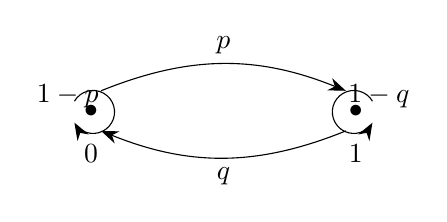
\begin{tikzpicture}[scale=1.05,>={Stealth[length=2.2mm]}]
  \node (A) at (0,0) {$\bullet$};
  \node[below=1mm] at (A.south) {$0$};
  \node (B) at (3.2,0) {$\bullet$};
  \node[below=1mm] at (B.south) {$1$};
  \draw[->] ($(A.north)+(0.12,0.05)$) to[bend left=22] node[above]{$p$} ($(B.north)+(-0.12,0.05)$);
  \draw[->] ($(B.south)+(-0.12,-0.05)$) to[bend left=22] node[below]{$q$} ($(A.south)+(0.12,-0.05)$);
  \draw[->] (A.150) arc[start angle=150,end angle=-150,radius=2.6mm] node[pos=0.35,left]{$1-p$};
  \draw[->] (B.30) arc[start angle=30,end angle=330,radius=2.6mm] node[pos=0.35,right]{$1-q$};
\end{tikzpicture}
\qquad
\text{考察轨道：}\ 0\cdots0\ 1\cdots1\ 0\cdots0\ 1\cdots1\ \cdots
\]
把轨道按游程分解：$0$-游程长 $\xi_1,\xi_2,\dots$，$1$-游程长 $\eta_1,\eta_2,\dots$，
则 $\xi_i,\eta_i$ 相互独立，$\xi_i$ i.i.d.\ $\sim G(p)$，$\eta_i$ i.i.d.\ $\sim G(q)$，
$L_i:=\xi_i+\eta_i$。令
\[
V_0(n):=\bigl|\{m\le n:X_m=0\}\bigr|
=\xi_1+\dots+\xi_r+\zeta_n ,\qquad 0\le\zeta_n\le\xi_{r+1},\ r=R_n ,
\]
其中 $\zeta_n$ 为当前未完成的游程（手写笔记记作 $\xi_n$）。于是
\[
\frac{V_0(n)}{n+1}
=\frac{\xi_1+\dots+\xi_{R_n}}{R_n}\cdot\frac{R_n}{n+1}+\frac{\zeta_n}{n+1}
\ \xrightarrow{\ \text{a.s.}\ }\ \E\xi\cdot\frac{1}{\E L}+0
=\frac{q}{p+q}=\pi_0 ,
\]
即 $\pi_0$ 为不变分布。
\end{example}

\paragraph{另考虑}
令 $n_1:=\inf\{n:X_n=0\}$，$n_i:=\inf\{n\ge n_{i-1}+1:X_n=0\}$，
$L_r:=n_r-n_{r-1}\ (r\ge2)$，$L_1:=n_1$，称为\textbf{更新间隔}，则 $\{L_r:r\ge2\}$ i.i.d.，
\[
\Pp(L_r=m)=
\begin{cases}
1-p, & m=1,\\
p\,(1-q)^{m-2}\,q, & m\ge2,
\end{cases}
\qquad
\E L_r=\frac{p+q}{q}=\frac{1}{\pi_0}.
\]
由更新定理即有
$\dfrac{V_0(n)}{n+1}\xrightarrow{\ \text{a.s.}\ }\dfrac{1}{\E L_r}=\pi_0$。 \qed

\secn{1.3}{状态的分类}

\begin{definition}[可达与互通]
若 $\Pp_i\bigl(\exists\,n\ge0,\ \text{s.t. }X_n=j\bigr)>0$，则称 $i$ \textbf{可达} $j$，记 $i\reach j$。
\end{definition}

\begin{itemize}
  \item $\Pp_i(\exists n\ge0,\ \text{s.t.}\ X_n=j)>0\iff \exists\,n,\ \text{s.t.}\ p_{ij}^{(n)}>0$。
        注意 $p_{ij}^{(n)}\le\Pp_i\bigl(\bigcup_{n\ge0}\{X_n=j\}\bigr)\le\sum_{n\ge0}p_{ij}^{(n)}$。
  \item $\exists\,n,\ \text{s.t.}\ p_{ij}^{(n)}>0\iff i=j$ 或
        （$j\ne i$ 时）$\exists\,n\ge1$ 及 $i_0,\dots,i_n=j$ 使
        $p_{i_0i_1}p_{i_1i_2}\cdots p_{i_{n-1}i_n}>0$。
\end{itemize}

\begin{definition}[互通与不可约]
若 $i\reach j$ 且 $j\reach i$，则称 $i,j$ \textbf{互通}，记 $i\comm j$。
若 $S$ 中任意 $i,j$ 互通，则称 $(P,S)$ 马氏链\textbf{不可约}。
互通类 $[i]:=\{j\in S:i\comm j\}$。
\end{definition}

\begin{definition}[闭集]
若 $\forall i\in A,\ j\notin A$，$p_{ij}=0$，则称 $A$ 是\textbf{闭的}。闭的互通类称为\textbf{闭类}。
\end{definition}

\begin{proposition}
若 $A$ 是互通类但不是闭的，则
$\Pp_i\bigl(\exists n\ge0,\ X_n\notin A\bigr)>0$，$\forall i\in A$。
\end{proposition}

\begin{remark}
若 $|A|<+\infty$，则上述概率为 $1$。若 $|A|=+\infty$ 则未必：考虑带吸收态的随机游动
（$0$ 为吸收态，$1,2,\dots$ 上向右概率 $p>q$）：
\[
p_i:=\Pp_i(\exists n,\ X_n=0)
\]
满足 $p_i=p\,p_{i+1}+q\,p_{i-1}$，解得 $p_i=\bigl(\tfrac{q}{p}\bigr)^i<1$，即从 $i$ 出发
可能永远不离开 $A=\{1,2,\dots\}$。
\end{remark}

\secn{1.4}{首达时与强马氏性}

\subsection*{1.4.1\quad 首达时与首入时}

轨道 $\vec{X}(\omega):=(X_0(\omega),X_1(\omega),\dots)$。

\begin{definition}
\textbf{首达时} $\tau_i(\omega):=\inf\{n\ge0:X_n(\omega)=i\}$，约定 $\inf\varnothing:=+\infty$；
\textbf{首入时} $\sigma_i(\omega):=\inf\{n\ge1:X_n(\omega)=i\}$。
\end{definition}

\subsection*{1.4.2\quad SRW 的首达时}

\begin{proposition}[反射原理]
\[
\Pp_0\bigl(\tau_i<n,\ S_n=i+j\bigr)=\Pp_0\bigl(\tau_i<n,\ S_n=i-j\bigr),
\qquad \forall j\ge1 .
\]
\end{proposition}

\begin{proof}
只需考虑 $1\le i<n$。对任意从 $i$ 出发到达 $i+j$ 的轨道（在时刻 $\tau_i$ 首次触及水平线
$i$），将 $\tau_i$ 之后的部分关于水平线 $S=i$ 反射，得到一条从 $i$ 到 $i-j$ 的轨道与之对应；
由 SRW 每条路径等概率即知二者概率相等。
\begin{center}
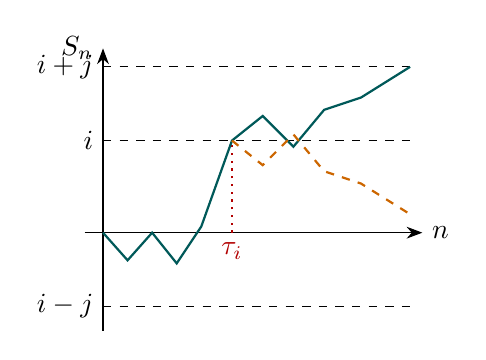
\begin{tikzpicture}[scale=0.78,>={Stealth[length=2mm]}]
  \draw[->] (-0.3,0)--(5.2,0) node[right]{$n$};
  \draw[->] (0,-1.6)--(0,3.0) node[left]{$S_n$};
  \draw[dashed] (0,1.5)--(5,1.5) node[pos=0,left]{$i$};
  \draw[dashed] (0,-1.2)--(5,-1.2) node[pos=0,left]{$i-j$};
  \draw[dashed] (0,2.7)--(5,2.7) node[pos=0,left]{$i+j$};
  \draw[red!70!black,thick,dotted] (2.1,0) -- (2.1,1.5) node[pos=0,below]{$\tau_i$};
  \draw[teal!70!black,thick]
    (0,0) -- (0.4,-0.45) -- (0.8,0.0) -- (1.2,-0.5) -- (1.6,0.1)
    -- (2.1,1.5) -- (2.6,1.9) -- (3.1,1.4) -- (3.6,2.0) -- (4.2,2.2) -- (5,2.7);
  \draw[orange!80!black,thick,dashed]
    (2.1,1.5) -- (2.6,1.1) -- (3.1,1.6) -- (3.6,1.0) -- (4.2,0.8) -- (5,0.3);
\end{tikzpicture}
\end{center}
\end{proof}

\begin{proposition}
$\Pp_0(\tau_i=n)=\dfrac{i}{n}\,\Pp_0(S_n=i)$。
\end{proposition}

\begin{proof}
易知在 RW 中 $n$ 与 $i$ 奇偶性相同。分解
\[
\{S_n=i\}=\{\tau_i=n\}\ \sqcup\ \{\tau_i<n,\ S_n=i\},
\]
后者 $=\{\tau_i<n,\,S_{n-1}=i+1,\,S_n=i\}\ \sqcup\ \{\tau_i<n,\,S_{n-1}=i-1,\,S_n=i\}$，
而这两个事件经反射一一对应于 $\{S_{n-1}=i+1,\ S_n=i\}$。故
\[
\Pp_0(S_n=i)=\Pp_0(\tau_i=n)+2\,\Pp_0(S_{n-1}=i+1,\ S_n=i),
\]
\[
\darr\quad \Pp_0(\tau_i=n)=\Pp_0(S_n=i)-\Pp_0(S_{n-1}=i+1)=\frac{i}{n}\,\Pp_0(S_n=i). \qed
\]
\end{proof}

\begin{proposition}
$\Pp_0\bigl(\tau_1>2n-1\bigr)=\Pp_0\bigl(S_{2n}=0\bigr)$。
\end{proposition}

\begin{proof}
由反射原理（取 $i=1$）：$\{\tau_1<2n,\ S_{2n}=1+j\}\ \leftrightarrow\ \{\tau_1<2n,\ S_{2n}=1-j\}$（$j\ge1$）；
又 $\{\tau_1<2n,\ S_{2n}=1-j\}\ \longleftrightarrow\ \{S_{2n}=1+j\}$
（终点 $\ge2$ 的轨道必先击中 $1$，反射还原）。对 $j\ge1$ 求和：
\[
\Pp_0(S_{2n}\ge2)=\Pp_0(\tau_1<2n,\ S_{2n}\le0),
\]
\[
\darr\quad \Pp_0(\tau_1<2n)=2\,\Pp_0(S_{2n}\ge2)=\Pp_0(S_{2n}\ne0),
\]
\[
\darr\quad \Pp_0(\tau_1>2n-1)=\Pp_0(S_{2n}=0). \qed
\]
\end{proof}

\begin{proposition}
$\Pp_0(\tau_i<+\infty)=1$；\quad
$\Pp_0(\sigma_0<+\infty)=1$；\quad
$\E_0\tau_i=\E_0\sigma_0=+\infty$.
\end{proposition}

\begin{proof}
$\Pp_0(\tau_1>2n-1)=\dbinom{2n}{n}2^{-2n}\sim\dfrac{1}{\sqrt{\pi n}}\to0$，故
$\Pp_0(\tau_1<\infty)=1$；而
\[
\E\tau_1=\sum_{n\ge1}\Pp_0(\tau_1>2n-1)+1=+\infty .
\]
由平移不变性 $\E_0\tau_i=+\infty$；且 $\sigma_0\ \doteq\ 1+\tau_1$
（$0\to\pm1\to\cdots\to0$，即先走一步再用 $\tau_1$ 型击中时间返回 $0$）。 \qed
\end{proof}

\begin{proposition}[反正弦律]
令
\[
E_n:=\max\bigl\{m\le n:\ S_m=0,\ S_{m+1}\ne0,\ S_{m+2}\ne0,\ \dots,\ S_n\ne0\bigr\}
\]
（前 $n$ 次中最后一次离开 $0$ 的时刻），则
\[
\lim_{n\to+\infty}\Pp_0\bigl(E_n\le\delta n\bigr)=\frac{2}{\pi}\arcsin\sqrt{\delta},
\qquad \delta\in(0,1).
\]
\end{proposition}

\begin{proof}
记 $m=\lfloor\delta n\rfloor$。则
\begin{align*}
\Pp_0(E_n\le\delta n)&=\Pp_0(S_r\ne0,\ \delta n<r\le n)\\
&=\sum_i\Pp_0(S_m=i)\,\Pp_i(\tau_0>n-m)
=1-\sum_i\Pp_0(S_m=i)\,\Pp_0(\tau_i\le n-m),
\end{align*}
其中对 $i\ge1$，
\[
\{\tau_i\le n-m\}=\{S_{n-m}=i\}\ \cup\ \{\tau_i<n-m,\ S_{n-m}>i\}\ \cup\ \{\tau_i<n-m,\ S_{n-m}<i\},
\]
\[
\darr\quad \Pp_0(\tau_i\le n-m)=\Pp_0(S_{n-m}=i)+2\,\Pp_0(S_{n-m}>i)
\qquad(i\ge1,\ \text{反射原理}).
\]
代回得
\[
\Pp_0(E_n\le\delta n)
=1-\sum_i\Pp_0(S_m=i)\Bigl[\Pp_0(S_{n-m}=i)+\Pp_0\bigl(|S_{n-m}|>|i|\bigr)\Bigr].
\]
第一项：$\sum_i\Pp_0(S_m=i)\Pp_0(S_{n-m}=i)\to0$（CLT，两项各 $\sim C/\sqrt{n}$）。

第二项：取 $\{T_{n-m}\}$ i.i.d.\ 且 $\{T_{n-m}\}\ \doteq\ \{S_{n-m}\}$，则
\[
\sum_i\Pp_0(S_m=i)\,\Pp_0\bigl(|T_{n-m}|>|i|\bigr)
=\Pp_0\bigl(|T_{n-m}|>|S_m|\bigr)
=\Pp_0\!\left(\frac{|T_{n-m}|/\sqrt{n-m}}{|S_m|/\sqrt{m}}>\sqrt{\frac{m}{n-m}}\right),
\]
由 CLT，右边的阈值 $\sqrt{m/(n-m)}\to\sqrt{\delta}/\sqrt{1-\delta}$，故上式趋于
\[
\Pp\left(\frac{|N(0,1)|}{|N(0,1)|}>\frac{\sqrt{\delta}}{\sqrt{1-\delta}}\right)
=1-\frac{2}{\pi}\arcsin\sqrt{\delta} .
\]
于是 $\Pp_0(E_n\le\delta n)\to1-\Bigl(1-\dfrac{2}{\pi}\arcsin\sqrt{\delta}\Bigr)
=\dfrac{2}{\pi}\arcsin\sqrt{\delta}$。 \qed
\end{proof}

\subsection*{1.4.3\quad 强马氏性}

记 $\tau=\tau_i$，设 $\Pp(\tau_i<+\infty)>0$。在 $\{\omega:\tau_i(\omega)<+\infty\}$ 上定义
\textbf{随机平移}：
\[
Y_m:=X_{\tau+m},
\qquad
(Y_0,Y_1,\dots):=\bigl(X_{\tau(\omega)}(\omega),\,X_{\tau(\omega)+1}(\omega),\,\dots\bigr).
\]
令 $\vec{Z}=(X_0,X_1,\dots,X_\tau)$，在 $\Pp(\,\cdot\mid\tau<+\infty)$ 下其值域为
$\bigcup_{n=0}^{+\infty}I_n$，其中
\[
I_n:=\bigl\{\vec{i}\in S^{\,n+1}:\ i_0,\dots,i_{n-1}\ne i,\ i_n=i\bigr\}.
\]
记 $\vec{X}^{(n)}=(X_0,X_1,\dots,X_n)$，则 $\forall\vec{i}\in I_n$，
$\{\vec{Z}=\vec{i}\}=\{\vec{X}^{(n)}=\vec{i}\}$，故
\[
\Pp(\vec{Z}=\vec{i})=\mu_{i_0}\,p_{i_0i_1}\cdots p_{i_{n-1}i},
\qquad
\Pp(\tau<+\infty)=\sum_{n=0}^{+\infty}\Pp(\tau=n)
=\sum_{n=0}^{+\infty}\sum_{\vec{i}\in I_n}\Pp\bigl(\vec{X}^{(n)}=\vec{i}\bigr),
\]
\[
\therefore\quad
\Pp\bigl(\vec{Z}=\vec{i}\mid\tau<+\infty\bigr)=\frac{\Pp(\vec{Z}=\vec{i})}{\Pp(\tau<+\infty)}.
\]

\begin{proposition}[强马氏性]
在 $\{\tau_i<+\infty\}$ 或 $\{\tau_i=n\}$ 条件下，$\{Y_m\}$ 是从 $i$ 出发的马氏链（转移矩阵
$P$），且与 $\vec{Z}$ 独立。
\end{proposition}

\begin{proof}
在 $\{\tau_i=n\}$ 条件下，$\vec{Z}=\vec{X}^{(n)}\in I_n$。记
$\vec{j}:=(j_0,j_1,\dots,j_m)$，$B:=\{\vec{Y}=\vec{j}\}$，$C:=\{\vec{Z}=\vec{i}\}$，
则只需证
\[
\Pp_{\mid\tau=n}(BC)=\ind{j_0=i}\,p_{j_0j_1}\cdots p_{j_{m-1}j_m}\cdot
\Pp_{\mid\tau=n}(C).
\]
记 $\widehat{B}:=\{(X_n,X_{n+1},\dots,X_{n+m})=\vec{j}\}$，
$\widehat{C}:=\{\vec{X}^{(n)}=\vec{i}\}$，$D:=\{\tau_i=n\}$。当 $\vec{i}\in I_n$ 时
$C=\widehat{C}\subseteq D$，$BD=\widehat{B}D$，于是
\[
BC=BD\,C=\widehat{B}D\,\widehat{C}=\widehat{B}\,\widehat{C}
\ \darr\quad
\Pp(BC)=\Pp(\widehat{B}\,\widehat{C})
=\ind{j_0=i}\,p_{j_0j_1}\cdots p_{j_{m-1}j_m}\cdot\Pp(\widehat{C}). \qquad\qed
\]
在 $\{\tau_i<+\infty\}$ 条件下：
\[
\Pp_{\mid\tau<+\infty}(BC)
=\frac{\sum_n\Pp_{\mid\tau=n}(BC)\,\Pp(\tau=n)}{\Pp(\tau<+\infty)}
=\frac{\sum_n(\ast)\,\Pp(\tau=n)}{\Pp(\tau<+\infty)} ,
\]
其中 $(\ast)$ 与 $n$ 无关，故上式 $=(\ast)$。 \qed
\end{proof}

\begin{corollary}
把 $\tau_i$ 换成 $\sigma_i$，强马氏性依然成立。
\end{corollary}

\begin{example}[SRW]
$\tau_i=\tau_1+(\tau_2-\tau_1)+\dots+(\tau_i-\tau_{i-1})$。由强马氏性，
$\tau_1,\ \tau_2-\tau_1,\ \dots,\ \tau_i-\tau_{i-1}$ i.i.d.

考虑（首步分析）$\E_0\tau_1=\tfrac12\times1+\tfrac12\bigl(1+\E_0\tau_2\bigr)$；
又 $\E_0\tau_2=2\,\E_0\tau_1$，故 $\E_0\tau_1=+\infty$。
\end{example}

\secn{1.5}{常返性}

$j\reach i$ 可达 $\iff \Pp_j(\tau_i<+\infty)>0$。本节回答：总共访问 $i$ 多少次？

\subsection*{1.5.1\quad 回访时间}

给定 $i$。$T_0:=0$；若 $T_{r-1}<+\infty$，则定义
\[
T_r:=\inf\{n\ge T_{r-1}+1:\ X_n=i\},
\qquad
\sigma_r:=T_r-T_{r-1}.
\]
$X_0=i$ 时 $T_1=\sigma_1$；$X_0\ne i$ 时 $T_1=\tau_1$。

\begin{proposition}
$\forall r\ge1$ 及 $m_1,m_2,\dots,m_r\ge1$：
\[
\Pp_i(\sigma_1=m_1,\ \sigma_2=m_2,\ \dots,\ \sigma_r=m_r)
=\prod_{k=1}^{r}\Pp_i(\sigma_k=m_k).
\]
注意：上式只有在 $\{\sigma_k<+\infty\}$ 条件下才代表独立。
\end{proposition}

\begin{proof}
记 $\vec{i}:=(i_0,i_1,\dots,i_n)$，
$J_n:=\{\vec{i}\in S^{\,n+1}:\ i_0=i_n=i,\ \text{中间分量}\ne i\}$，
$n_S:=\sum_{t=1}^{S}m_t$（$n_0:=0$），$\vec{Z}_S:=(X_{n_{S-1}},\dots,X_{n_S})$。
时间轴示意：
\begin{center}
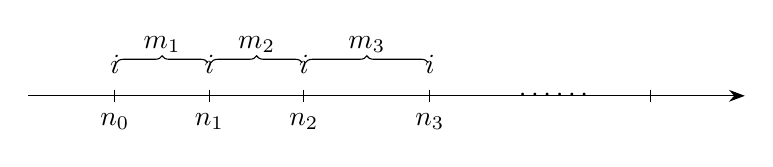
\begin{tikzpicture}[scale=1.0,>={Stealth[length=2mm]}]
  \draw[->] (-0.5,0)--(8.6,0);
  \foreach \x/\l in {0.6/$n_0$,1.8/$n_1$,3.0/$n_2$,4.6/$n_3$,7.4/}{
    \draw (\x,0.08)--(\x,-0.08);}
  \node[below] at (0.6,-0.1) {$n_0$};
  \node[below] at (1.8,-0.1) {$n_1$};
  \node[below] at (3.0,-0.1) {$n_2$};
  \node[below] at (4.6,-0.1) {$n_3$};
  \node at (6.2,0) {$\cdots\cdots$};
  \draw[decorate,decoration={brace}] (0.62,0.42)--(1.78,0.42) node[midway,above]{$m_1$};
  \draw[decorate,decoration={brace}] (1.82,0.42)--(2.98,0.42) node[midway,above]{$m_2$};
  \draw[decorate,decoration={brace}] (3.02,0.42)--(4.58,0.42) node[midway,above]{$m_3$};
  \node[above] at (0.6,0.16) {$i$};
  \node[above] at (1.8,0.16) {$i$};
  \node[above] at (3.0,0.16) {$i$};
  \node[above] at (4.6,0.16) {$i$};
\end{tikzpicture}
\end{center}
则
\[
\Pp(\sigma_1=m_1,\ \sigma_2=m_2,\ \dots,\ \sigma_r=m_r)
=\sum_{\substack{i_k\in J_{m_k}\\ k=1,\dots,r}}
\Pp_i\bigl(\vec{Z}_1=\vec{i}_1,\ \vec{Z}_2=\vec{i}_2,\ \dots,\ \vec{Z}_r=\vec{i}_r\bigr)
\]
\[
\xrightarrow{\ \text{马氏性}\ }
\sum\Pp_i\bigl(\vec{X}^{(m_1)}=\vec{i}_1\bigr)\cdots
\Pp_i\bigl(\vec{X}^{(m_r)}=\vec{i}_r\bigr)
=\prod_{s=1}^{r}\sum_{\vec{i}_s\in J_{m_s}}
\Pp_i\bigl(\vec{X}^{(m_s)}=\vec{i}_s\bigr)
=\prod_{s=1}^{r}\Pp_i(\sigma_s=m_s). \qed
\]
\end{proof}

\begin{proposition}
记 $\rho_i:=\Pp_i(\sigma_i<+\infty)$，则 $\Pp_i(T_r<+\infty)=\rho_i^{\,r}$。
\end{proposition}

\begin{proof}
归纳法。$r=1$ 时 $T_1=\sigma_1$，故成立。一般地
\[
\Pp_i(T_r<+\infty)
=\Pp_i\bigl(T_r<+\infty\mid T_1<+\infty,\dots,T_{r-1}<+\infty\bigr)\cdot
\Pp_i(T_1<+\infty,\dots,T_{r-1}<+\infty)
\]
\[
\xrightarrow{\ \text{强马氏性}\ }
\rho_i\cdot\rho_i^{\,r-1}=\rho_i^{\,r}. \qed
\]
\end{proof}

\subsection*{1.5.2\quad 回访总次数}

\[
V_i:=\sum_{n=0}^{+\infty}\ind{X_n=i}.
\]
则 $\Pp_i(V_i\ge r+1)=\Pp_i(T_r<+\infty)=\rho_i^{\,r}$，即 $V_i$ 服从几何分布。故：

\[
\boxed{\ \rho_i=1\iff\Pp_i(V_i=+\infty)=1\ \text{（常返）};\qquad
0<\rho_i<1\iff\Pp_i(V_i<+\infty)=1.\ }
\]
由 $V_i\sim$ 几何分布：
\[
\E_iV_i=
\begin{cases}
+\infty, & \rho_i=1,\\[0.2em]
\dfrac{1}{1-\rho_i}<+\infty, & 0<\rho_i<1.
\end{cases}
\]

\begin{proposition}
设 $i$ 常返，$X_0=i$。记 $\vec{Z}^{(r)}:=(X_{T_{r-1}},\dots,X_{T_r})$，则
$\vec{Z}^{(1)},\vec{Z}^{(2)},\dots$ i.i.d.
\end{proposition}

\subsection*{1.5.3\quad 常返与互通类}

\begin{proposition}
设 $i$ 常返，$i\reach j$，则
（1）$j\reach i$ 且 $j$ 常返；
（2）$\Pp_i(V_j=+\infty)=\Pp_j(V_i=+\infty)=1$；
（3）$\Pp_i(\tau_j<+\infty)=\Pp_j(\tau_i<+\infty)=1$。
\end{proposition}

\begin{proof}
（2）⇒（3）显然（$V_j=+\infty$ 时必有 $\tau_j<+\infty$）。只需证（1）（2）。

先证（2）（i）$\Pp_i(V_j=+\infty)=1$：取 $X_0=i$，$\vec{Z}^{(1)},\vec{Z}^{(2)},\dots$ i.i.d.，
令 $A_r:=\{\vec{Z}^{(r)}\ \text{中含有}\ j\}$。则 $A_r$ i.i.d.，且
$\Pp_i(\tau_j<+\infty)>0$、$\{\tau_j<+\infty\}\subseteq\bigcup_rA_r$，故
$p:=\Pp(A_r)>0$。由 SLLN：
$\tfrac1r\sum_r\ind{A_r}\to\E\ind{A_r}=p\ \darr\ \sum_r\ind{A_r}\to+\infty$，
即 $A_1,A_2,\dots$ 必定发生无穷多次，$\Pp_i(V_j=+\infty)=1$。

（2）（ii）$\Pp_j(V_i=+\infty)=1$：由（i）$\Pp_i(\tau_j<+\infty)=1$。令 $X_0=i$，
$Y_n:=X_{\tau_j+n}$，则（注意 $\tau_j<+\infty$ a.s.，且 $\tau_j$ 之前对 $i$ 的访问至多
$\tau_j$ 次，而 $X_0=i$ 贡献一次）
\[
1+V_i^{(Y)}\ \le\ V_i\ \le\ V_i^{(Y)}+\tau_j
\ \darr\quad \{V_i=+\infty\}=\{V_i^{(Y)}=+\infty\},
\]
\[
\darr\quad 1=\Pp_i(V_i=+\infty)=\Pp_i\bigl(V_i^{(Y)}=+\infty\bigr)
\xrightarrow{\ \text{强马氏性}\ }\Pp_j(V_i=+\infty).
\]
（1）由（2）（ii）$\Pp_j(\tau_i<+\infty)=1$。令 $X_0=j$，$Y_n:=X_{\tau_i+n}$，则
$\{V_j=+\infty\}=\{V_j^{(Y)}=+\infty\}$，故
\[
\Pp_j(V_j=+\infty)=\Pp_j\bigl(V_j^{(Y)}=+\infty\bigr)
\xrightarrow{\ \text{强马氏性}\ }\Pp_i(V_j=+\infty)=1,
\]
且 $j\reach i$，$j$ 常返。 \qed
\end{proof}

\secn{1.6}{击中概率}

\subsection*{1.6.1\quad 首步分析法}

\begin{example}[赌徒破产模型]
SRW，$\tau=\tau_0\wedge\tau_N$。则 $\Pp(\tau_0<+\infty,\ \tau_N<+\infty)=1$。令
$x_k:=\Pp_k(\tau_N<\tau_0)$，由首步分析
\[
x_k=\tfrac12x_{k+1}+\tfrac12x_{k-1},
\qquad x_0=0,\ x_N=1
\ \darr\quad x_k=\frac{k}{N}.
\]
\end{example}

一般马氏链。固定 $0\in S$，$x_i:=\Pp_i(\tau_0<+\infty)$，则
\begin{equation}
x_i=\sum_{j\in S}p_{ij}x_j,\quad\forall i\ne0;
\qquad x_0=1.
\tag{$\ast$}
\end{equation}
固定 $D\subseteq S$，$x_i:=\Pp_i(\tau_D<+\infty)$，则
\begin{equation}
x_i=\sum_{j\in S}p_{ij}x_j,\quad\forall i\notin D;
\qquad x_i=1,\quad\forall i\in D.
\tag{$\ast$}
\end{equation}
称 $x_i=\Pp_i(\tau_0<+\infty)$ 为\textbf{从 $i$ 出发到 $0$ 的击中概率}。

\begin{proposition}
击中概率是方程 $(\ast)$ 的最小非负解。
\end{proposition}

\begin{definition}
称满足 $p_{ii}=1$ 的状态 $i$ 为\textbf{吸收态}。设 $D\subseteq S$ 为闭集，
$\Pp_j(\tau_D<+\infty)$ 称为\textbf{从 $j$ 出发被 $D$ 吸收的概率}。
\end{definition}

\begin{question}
$\tau_D$ 的分布？$\Pp_i(\tau_D=k)=?$\quad
$i\in D$ 时 $\Pp_i(\tau_D=0)=1$；$i\in D^c$ 时留作讨论。
\end{question}

\subsection*{1.6.2\quad 判别常返性}

设 $S$ 不可约（$S$ 互通），给定 $0\in S$。则
\[
\rho_0=\Pp_0(\sigma_0<+\infty)=\sum_i p_{0i}\,\Pp_i(\tau_0<+\infty),
\]
且 $0$ 常返 $\iff\rho_0=1\iff \Pp_i(\tau_0<+\infty)=1,\ \forall i\in S$。

\begin{proposition}
常返 $\iff$ 方程组
\[
\begin{cases}
x_i=\sum_{j\in S}p_{ij}x_j, & \forall i\ne0,\\
x_0=1
\end{cases}
\]
在 $[0,1]$ 上只有恒为 $1$ 的解。
\end{proposition}

\begin{example}[生灭链的常返性]
$S=\Z^+$，$p_{i,i+1}=b_i$，$p_{i,i-1}=d_i$，$b_i+d_i=1$，$b_0=1$。
令 $x_i=\Pp_i(\tau_0<+\infty)$，则
\[
x_i=b_ix_{i+1}+d_ix_{i-1}\qquad(i\ge1).
\]
解：令 $R_i:=1+\sum_{k=1}^{i}\dfrac{d_1\cdots d_k}{b_1\cdots b_k}$，$R_0:=1$，则
\[
R_i\,(1-x_1)=1-x_{i+1}\qquad(i\ge0);
\qquad
R:=1+\sum_{k\ge1}\frac{d_1\cdots d_k}{b_1\cdots b_k}.
\]
于是 $R<+\infty$ 时可构造 $x_1=1-\dfrac1R$（此时 $1-x_{i+1}=\dfrac{R_i}{R}\in[0,1]$），
非常返；$R=+\infty$ 时有且仅有唯一解 $x_i\equiv1$，常返。 \qed
\end{example}

\begin{remark}[两端生灭链]
$S=\Z$，$p_{i,i+1}=p$，$p_{i,i-1}=q$。只有 $p=q$ 时常返。

$p>q$ 时 $\Pp_0(\tau_1<+\infty)=1$。考虑 $x:=\Pp_0(\tau_{-1}<+\infty)$，首步分析：
\[
x=q\cdot1+p\cdot\Pp_1(\tau_{-1}<+\infty)=q+p\,x^2
\ \darr\quad x=1\ \text{或}\ \frac{q}{p}.
\]
因 $\tfrac qp<1$，故 $\tfrac qp$ 是击中概率，非常返。
\end{remark}

\begin{example}[规则树 $\mathbb{T}^d$ 上的 $\lambda$-biased RW]
\[
p_{ij}=
\begin{cases}
\dfrac{\lambda}{\lambda+d}, & j\ \text{是}\ i\ \text{的父结点},\\[0.5em]
\dfrac{1}{\lambda+d}, & j\ \text{是}\ i\ \text{的子结点},
\end{cases}
\qquad
p_{0j}:=\frac1d .
\]
\begin{center}
\begin{tikzpicture}[scale=0.9]
  \node[circle,fill,inner sep=1.1pt,label=right:$i_0$] (root) at (0,1.4) {};
  \node[circle,fill,inner sep=1.1pt,label=left:$i$] (i) at (-0.9,0.5) {};
  \node[circle,fill,inner sep=1.1pt] (r2) at (0.9,0.5) {};
  \node[circle,fill,inner sep=1.1pt,label=left:$i_1$] (i1) at (-1.35,-0.4) {};
  \node[circle,fill,inner sep=1.1pt,label=right:$i_2$] (i2) at (-0.45,-0.4) {};
  \draw (root)--(i) (root)--(r2) (i)--(i1) (i)--(i2);
  \node at (2.6,0.4) {（例：$d=2$）};
\end{tikzpicture}
\end{center}
球对称性：$|i|=|j|\ \darr\ \Pp_i(\tau_0<+\infty)=\Pp_j(\tau_0<+\infty)=:a_{|i|}$。于是
\[
a_0=1,\qquad
a_n=\frac{\lambda}{\lambda+d}\,a_{n-1}+\frac{d}{\lambda+d}\,a_{n+1}\quad(n\ge1),
\]
\[
\darr\quad
a_0-a_n=(a_0-a_1)\Bigl(1+\frac{\lambda}{d}+\frac{\lambda^2}{d^2}+\dots+\frac{\lambda^{n-1}}{d^{n-1}}\Bigr).
\]
故 $\lambda<d$ 时，取 $a_0-a_1=1-\dfrac{\lambda}{d}$ 得 $a_n=\bigl(\dfrac{\lambda}{d}\bigr)^n$，
从而即知非常返；$\lambda\ge d$ 时 $a_n\equiv1$，故常返。 \qed
\end{example}

\secn{1.7}{格林函数}

\subsection*{1.7.1\quad 判别常返性}

对 $i,j\in S$，定义
\[
G_{ij}:=\E_iV_j=\E_i\sum_{n\ge0}\ind{X_n=j}
\xrightarrow{\ \text{Fubini}\ }
\sum_{n\ge0}\E_i\ind{X_n=j}=\sum_{n\ge0}p_{ij}^{(n)},
\]
称为 \textbf{Green 函数}。

\begin{proposition}
$i$ 常返 $\iff G_{ii}=+\infty$（by definition）。
\end{proposition}

\begin{example}[$d$ 维 SRW]
\textbf{$d=1$：}$p_{00}^{(2n+1)}=0$，
\[
p_{00}^{(2n)}=\frac{(2n)!}{n!\,n!}\cdot\frac{1}{2^{2n}}\sim\frac{1}{\sqrt{\pi n}},
\qquad
G_{00}=\sum_n p_{00}^{(n)}=+\infty,\ \text{故常返}.
\]

\textbf{$d=2$：}
\[
p_{00}^{(2n)}=\sum_{n_1+n_2=n}\frac{(2n)!}{(n_1!\,n_2!)^2}\cdot\frac{1}{4^{2n}}
=\binom{2n}{n}\cdot\frac{1}{2^{2n}}\cdot
\Bigl(\sum_{m=0}^{n}\binom{n}{m}\binom{n}{n-m}\Bigr)\cdot\frac{1}{2^{2n}}
=\Bigl(\binom{2n}{n}\cdot\frac{1}{2^{2n}}\Bigr)^{2}
\sim\frac{1}{\pi n},
\]
故常返。

\textbf{$d\ge3$：}$G_{00}\sim\sum_n n^{-d/2}<+\infty$，非常返。

例如 $d=3$（先确定各方向步数的分配 $n_1+n_2+n_3=n$）：
\[
p_{00}^{(2n)}=\sum_{n_1+n_2+n_3=2n}\frac{(2n)!}{(n_1!\,n_2!\,n_3!)^2}\cdot\frac{1}{6^{2n}}
=\sum_{n_1+n_2+n_3=n}\frac{(2n)!}{(2n_1)!\,(2n_2)!\,(2n_3)!}\cdot\frac{1}{3^{2n}}
\prod_{k=1}^{3}\binom{2n_k}{n_k}\frac{1}{2^{2n_k}}
\sim \frac{c}{n^{3/2}},
\]
故 $G_{00}<+\infty$，非常返。
\end{example}

\subsection*{1.7.2\quad 格林函数的其他应用}

\begin{proposition}
设 $i\reach j$，$i$ 常返，则 $j$ 常返。
\end{proposition}

\begin{proof}
前面已证 $i\reach j\ \darr\ j\reach i$。而
\[
i\comm j\iff \exists\,m,n\ge0:\ p_{ij}^{(n)}>0,\ p_{ji}^{(m)}>0,
\]
\[
p_{jj}^{(m+r+n)}=\sum_{k,l}p_{jk}^{(m)}p_{kl}^{(r)}p_{lj}^{(n)}
\ \ge\ p_{ji}^{(m)}\,p_{ii}^{(r)}\,p_{ij}^{(n)} .
\]
对 $r$ 求和得 $G_{jj}=+\infty$。 \qed
\end{proof}

\begin{proposition}
$G_{ij}=\Pp_i(\tau_j<+\infty)\cdot G_{jj}$\quad（$\darr\ G_{ij}\le G_{jj}$）。
\end{proposition}

\begin{proof}
只考虑 $i\ne j$。$V_j:=\sum_{n\ge0}\ind{X_n=j}$。若 $\tau_j=+\infty$，则 $V_j=0$；
若 $\tau_j<+\infty$，则强马氏性成立：令 $Y_n:=X_{\tau_j+n}$，则 $V_j=V_j^{(Y)}$，于是
\[
\Pp_i(V_j=m)=\Pp_i\bigl(V_j^{(Y)}=m,\ \tau_j<+\infty\bigr)
=\Pp_j(V_j=m)\cdot\Pp_i(\tau_j<+\infty),
\]
\[
\darr\quad
G_{ij}=\E_iV_j=\sum_{m\ge1}m\,\Pp_i(V_j=m)
=\sum_{m\ge1}m\,\Pp_j(V_j=m)\cdot\Pp_i(\tau_j<+\infty)
=\Pp_i(\tau_j<+\infty)\cdot G_{jj}. \qed
\]
\end{proof}

\begin{corollary}
若 $j$ 非常返，则 $\forall i$：$p_{ij}^{(n)}\to0\ (n\to+\infty)$。
\end{corollary}

\begin{proof}
$G_{ij}\le G_{jj}<+\infty$ 且 $G_{ij}=\sum_{n\ge0}p_{ij}^{(n)}$，故通项趋于 $0$。 \qed
\end{proof}

\begin{corollary}
设 $\pi$ 为不变分布，$j$ 非常返，则 $\pi_j=0$。
\end{corollary}

\begin{proof}
$G_{ij}\le G_{jj}<+\infty$，故
\[
\pi_iG_{ij}\le\pi_iG_{jj}
\ \darr\quad
\sum_i\pi_iG_{ij}\le G_{jj}<+\infty .
\]
而
\[
\sum_i\pi_iG_{ij}=\sum_i\pi_i\sum_{n\ge0}p_{ij}^{(n)}
=\sum_{n\ge0}\sum_i\pi_ip_{ij}^{(n)}
=\sum_{n\ge0}\pi_j
\begin{cases}
=+\infty, & \pi_j>0,
\end{cases}
\]
矛盾，故 $\pi_j=0$。 \qed
\end{proof}

\subsection*{1.7.3\quad 有限区域上的 Green 函数}

设 $D\subseteq S$，$\tau:=\tau_{D^c}$（首次离开 $D$ 的时刻），定义
\[
G_{ij}^{(D)}:=\E_i\sum_{n=0}^{\tau-1}\ind{X_n=j},\qquad i,j\in D,
\]
即限制在 $D$ 上的 Green 函数；$G_{ij}^{(S)}=G_{ij}$。

固定 $0\in D$，$x_i:=G_{i0}^{(D)}$ 满足
\[
\begin{cases}
x_i=\sum_{j\in S}p_{ij}x_j, & \forall i\in D\setminus\{0\},\\[0.2em]
x_0=1+\sum_{j\in S}p_{0j}x_j, &\\[0.2em]
x_i=0, & i\in D^c.
\end{cases}
\]

\begin{example}
设 $\{S_n\}$ 是一维 SRW，$N\ge3$，$D=\{1,2,\dots,N-1\}$，则
\[
G_{ij}^{(D)}=
\begin{cases}
\dfrac{2}{N}\,i\,(N-j), & 0<i\le j<N,\\[0.5em]
\dfrac{2}{N}\,j\,(N-i), & 0<j<i<N.
\end{cases}
\]
\end{example}

\begin{proof}
固定 $j$，$x_i:=G_{ij}^{(D)}$ 满足
\[
\begin{cases}
x_i=\frac12x_{i-1}+\frac12x_{i+1}, & 0<i<N,\ i\ne j,\\
x_j=1+\frac12x_{j-1}+\frac12x_{j+1}, &\\
x_0=x_N=0. &
\end{cases}
\]
故 $x_i$ 为分段等差数列：$x_i-x_{i-1}=x_{i+1}-x_i\ (i\ne j)$，于是
\[
x_{j-1}=(j-1)\,x_1,\qquad x_{j+1}=(N-j-1)\,x_{N-1},
\qquad
x_j=j\,x_1=(N-j)\,x_{N-1}
\ \darr\quad x_{N-1}=\frac{j}{N-j}\,x_1 .
\]
代入 $x_j=1+\frac12x_{j-1}+\frac12x_{j+1}$ 可解得 $x_1=\dfrac2N(N-j)$，从而即得 $x_i$。 \qed
\end{proof}

\begin{proposition}
$\tau:=\tau_{D^c}$，则 $\E_i\tau=\sum_{j\in D}G_{ij}^{(D)}$。
\end{proposition}

\begin{proof}
\[
\text{RHS}=\sum_{j\in D}\E_i\sum_{n=0}^{\tau-1}\ind{X_n=j}
=\E_i\sum_{n=0}^{\tau-1}\sum_{j\in D}\ind{X_n=j}.
\]
而 $\sum_{j\in D}\ind{X_n=j}=1,\ \forall n$（任意时刻必在且仅在一个点上），故 RHS $=\E_i\tau$。 \qed
\end{proof}

$y_i:=\E_i\tau$ 满足
\[
y_i=1+\sum_{j\in S}p_{ij}y_j,\quad\forall i\in D;
\qquad
y_i=0,\quad\forall i\in D^c .
\]
只需解之即可推出 Green 函数。

\begin{example}
在 SRW 中求 $\E_i(\tau_0\wedge\tau_N)$，$0<i<N$。

\textbf{方法 1.} $\E_i(\tau_0\wedge\tau_N)=\E_i\tau_{D^c}=\sum_{j\in D}G_{ij}^{(D)}
=\sum_{j=1}^{i}\frac2Nj(N-i)+\sum_{j=i+1}^{N-1}\frac2Ni(N-j)=i(N-i)$.

\textbf{方法 2.} $y_i:=\E_i(\tau_0\wedge\tau_N)$：
\[
y_i=1+\tfrac12y_{i+1}+\tfrac12y_{i-1}\quad(1\le i\le N-1),
\qquad y_0=y_N=0
\ \darr\quad y_i=i(N-i)
\]
（二阶等差数列）。
\end{example}

\subsection*{1.7.4\quad 瓦尔德等式}

SRW，$S_0=0$，$\tau:=\tau_j\wedge\tau_{-i}$。$S_\tau$ 的分布：
\[
\Pp_0(S_\tau=j)=\frac{i}{i+j}=\Pp_i(\tau_{i+j}<\tau_0),
\qquad
\Pp_0(S_\tau=-i)=\frac{j}{i+j}.
\]
于是 $\E_0S_\tau=0$，$\E_0S_\tau^2=ij$。注意 $\E_0S_\tau^2=\E_0\tau$。

\begin{proposition}[Wald 等式]
设 $\E\tau<+\infty$，$\E|\xi_1|<+\infty$，$\xi_i$ i.i.d.，$S_n:=\xi_1+\dots+\xi_n$（$n\ge1$），则：
\begin{enumerate}
  \item $\E S_\tau=\E\tau\cdot\E\xi_1$；
  \item 若 $\E\xi_1^2<+\infty$，$\E\xi_1=0$，则 $\E S_\tau^2=\E\tau\cdot\E\xi_1^2$。
\end{enumerate}
\end{proposition}

\secn{1.8}{遍历定理与正常返}

本节假设马氏链不可约。

\subsection*{1.8.1\quad 频率的极限}

\begin{proposition}
$\forall i\in S$：
\[
\Pp_\mu\Bigl(\lim_{n\to+\infty}\frac{V_i(n)}{n}=\frac{1}{\E_i\sigma_i}\Bigr)=1,
\qquad
V_i(n):=\sum_{m=0}^{n-1}\ind{X_m=i}.
\]
\end{proposition}

\begin{proof}
若 $i$ 非常返，则 $\E_i\sigma_i=+\infty$，且 $\lim_{n\to\infty}V_i(n)<+\infty$ a.s.，故结论正确。

若 $i$ 常返：$X_0=i$ 时即更新定理；$X_0=j\ne i$ 时，由 $\Pp_j(\tau_i<+\infty)=1$，
可从 $\tau_i$ 处取马氏链 $Y_n:=X_{\tau_i+n}$，对 $Y_n$ 用更新定理；再由
$V_i(n)=V_i^{(Y)}(n-\tau_i)$，
\[
\frac1nV_i(n)=\frac{n-\tau_i}{n}\cdot\frac{V_i^{(Y)}(n-\tau_i)}{n-\tau_i}
\ \longrightarrow\ \frac{1}{\E_i\sigma_i}\quad\text{a.s.}
\]
而 $\Pp_\mu(\ \cdot\ )=\sum_j\mu_j\Pp_j(\ \cdot\ )$，从而即证。 \qed
\end{proof}

\begin{proposition}
设 $\pi$ 为 $P$ 的不变分布，则 $\forall i\in S$：$\pi_i>0$，且
$\pi_i=\dfrac{1}{\E_i\sigma_i}$
\quad（$\darr\ \sum_{i\in S}\dfrac{1}{\E_i\sigma_i}=1$）。
\end{proposition}

\begin{proof}
先证 $\pi_i>0\ \forall i\in S$：取 $0\in S$ 使 $\pi_0>0$。因 $S$ 不可约，故 $\exists\,n$，
$p_{0i}^{(n)}>0$，于是
\[
\pi_i=\sum_j\pi_jp_{ji}^{(n)}\ \ge\ \pi_0\,p_{0i}^{(n)}>0,\qquad\forall i\in S.
\]
又由上一命题，$\dfrac{V_i(n)}{n}\to\dfrac{1}{\E_i\sigma_i}$ a.s.（在 $\Pp_\pi$ 意义下），
由有界收敛定理 $\E_\pi\dfrac{V_i(n)}{n}\to\dfrac{1}{\E_i\sigma_i}$。

下证 $\E_\pi\dfrac{V_i(n)}{n}=\pi_i$：
\[
\E_\pi\frac1nV_i(n)=\E_\pi\frac1n\sum_{m=0}^{n-1}\ind{X_m=i}
=\frac1n\sum_{m=0}^{n-1}\E_\pi\ind{X_m=i}
=\frac1n\sum_{m=0}^{n-1}\pi_i=\pi_i .
\]
故结论成立。 \qed
\end{proof}

\begin{corollary}
不可约马氏链的不变分布若存在则唯一。
\end{corollary}

\subsection*{1.8.2\quad 正常返}

若 $\E_i\sigma_i<+\infty$，则称 $i$ \textbf{正常返}；
若 $\Pp_i(\sigma_i<+\infty)=1$ 但 $\E_i\sigma_i=+\infty$，则称\textbf{零常返}。

取定 $0\in S$，定义
\[
\mu_i:=\E_0\sum_{n=0}^{\sigma_0-1}\ind{X_n=i},
\qquad \mu_0=1 .
\]
直观：$\mu_i$ 为一个回复周期内 $i$ 出现的次数；且
$\dfrac{\mu_i}{\E_0\sigma_0}=\dfrac{1}{\E_i\sigma_i}=\pi_i$。

\begin{proposition}
设 $0$ 常返，则 $\mu$ 是不变测度。
\end{proposition}

\begin{proof}
\[
\mu_j=\E_0\sum_{n=0}^{\sigma_0-1}\ind{X_n=j}
=\E_0\sum_{n=0}^{+\infty}\ind{X_n=j,\ n<\sigma_0}
=\sum_{n=0}^{+\infty}\Pp_0(n<\sigma_0,\ X_n=j).
\]
故
\[
\sum_j\mu_jp_{ji}
=\sum_j\sum_{n=0}^{+\infty}\Pp_0(n<\sigma_0,\ X_n=j,\ X_{n+1}=i)
=\sum_{n=0}^{+\infty}\sum_j\Pp(\ast)
=\sum_{n=0}^{+\infty}\Pp_0(n<\sigma_0,\ X_{n+1}=i)
\]
\[
=\E_0\sum_{n=0}^{+\infty}\ind{X_{n+1}=i,\ n<\sigma_0}
=\E_0\sum_{n=1}^{\sigma_0}\ind{X_n=i}
=\E_0\sum_{n=0}^{\sigma_0-1}\ind{X_n=i}=\mu_i .
\]
上式成立的原因：$i\ne0$ 时 $X_0=X_{\sigma_0}=0$，不影响求和；$\sigma_0<+\infty$ 且 $i=0$ 时
$X_0=X_{\sigma_0}=0$，不影响求和；$\sigma_0=+\infty$ 且 $i=0$ 时会差一项。故题设条件要求
$0$ 常返。 \qed
\end{proof}

\begin{theorem}
设 $P$ 不可约，则下列叙述等价：
（1）$\forall i\in S$，$i$ 正常返；（2）$\exists\,0\in S$，$0$ 正常返；（3）存在不变分布。
\end{theorem}

\begin{proof}
（1）$\Rightarrow$（2）显然。

（2）$\Rightarrow$（3）由上一命题知存在不变测度
$\mu_i:=\E_0\sum_{n=0}^{\sigma_0-1}\ind{X_n=i}$，而
\[
\sum_{i\in S}\mu_i=\sum_{i\in S}\E_0\sum_{n=0}^{\sigma_0-1}\ind{X_n=i}
=\E_0\sum_{n=0}^{\sigma_0-1}\sum_{i\in S}\ind{X_n=i}
=\E_0\sigma_0<+\infty,
\]
故可归一化。

（3）$\Rightarrow$（1）$\pi_i=\dfrac{1}{\E_i\sigma_i}>0$，故 $\E_i\sigma_i<+\infty$，
$\forall i\in S$，故 $S$ 正常返。 \qed
\end{proof}

\begin{corollary}
设 $S$ 有限且不可约，则存在不变分布。
\end{corollary}

\begin{proof}
$\frac1n\sum_{m=0}^{n-1}\ind{X_m=i}\to\dfrac{1}{\E_i\sigma_i}$ a.s.。因 $S$ 有限，
上式对 $i$ 求和得
\[
\sum_{i\in S}\frac{1}{\E_i\sigma_i}
\xleftarrow{\ \text{a.s.}\ }
\sum_{i\in S}\frac1n\sum_{m=0}^{n-1}\ind{X_m=i}
=\frac1n\sum_m\sum_i\ind{X_m=i}=1 .
\]
故 $\exists\,i\in S$，$\E_i\sigma_i<+\infty\ \darr\ i$ 正常返 $\darr$ 存在不变分布。 \qed
\end{proof}

\begin{lemma}
设 $P$ 不可约、常返，则 $\mu_i:=\E_0\sum_{n=0}^{\sigma_0-1}\ind{X_n=i}$
是（归一化 $\mu_0=1$ 下的）不变方程的唯一解。
\end{lemma}

\begin{proposition}
设 $P$ 不可约，若存在不可归一化的不变测度，则不变分布不存在。
\end{proposition}

\begin{proof}
若 $P$ 非常返，则若存在不变分布必有 $\pi_i=0\ \forall i$，故而矛盾。

若 $P$ 常返，则由引理的唯一性即知不存在不变分布。 \qed
\end{proof}

\subsection*{1.8.3\quad 遍历定理}

设 $P$ 不可约、正常返，则
\[
\frac1n\sum_{m=0}^{n-1}\ind{X_m=i}\ \longrightarrow\ \frac{1}{\E_i\sigma_i}=\pi_i
\quad\text{a.s.};
\qquad
\text{BCT}\ \darr\quad
\frac1n\sum_{m=0}^{n-1}\Pp_\mu(X_m=i)\ \longrightarrow\ \pi_i,\quad\forall\mu .
\]

\begin{lemma}[Scheffé]
设 $\lim_n\pi_i^{(n)}=\pi_i$，$\{\pi_i^{(n)}\}_i$、$\{\pi_i\}_i$ 均是分布列，则
\[
\lim_{n\to+\infty}\sum_{i\in S}\bigl|\pi_i^{(n)}-\pi_i\bigr|=0 .
\]
\end{lemma}

\begin{proposition}
设 $P$ 不可约、正常返，$\pi$ 是不变分布，则
\begin{enumerate}
  \item $\displaystyle\sum_{i\in S}\Bigl|\frac1n\sum_{m=0}^{n-1}p_{ji}^{(m)}-\pi_i\Bigr|\ \longrightarrow\ 0$；
  \item $\displaystyle\sum_{i\in S}\Bigl|\frac1n\sum_{m=0}^{n-1}\Pp_\mu(X_m=i)-\pi_i\Bigr|\ \longrightarrow\ 0$
        \quad（分布意义）；
  \item $\displaystyle\sum_{i\in S}\Bigl|\frac{V_i(n)}{n}-\pi_i\Bigr|\ \xrightarrow{\ \text{a.s.}\ }\ 0$
        \quad（轨道意义）.
\end{enumerate}
\end{proposition}

\begin{theorem}[遍历定理]
设 $P$ 不可约、正常返，$\sum_i\pi_i|f(i)|<+\infty$，则
\[
\Pp_\mu\Bigl(\lim_{n\to+\infty}\frac1n\sum_{m=0}^{n-1}f(X_m)=\sum_i\pi_if(i)\Bigr)=1 .
\]
\end{theorem}

\begin{proof}
先考虑直观：$\frac1n\sum_{m=0}^{n-1}f(X_m)=\frac1n\sum_{m=0}^{n-1}\sum_i f(i)\ind{X_m=i}
=\sum_i f(i)\cdot\frac1n\sum_{m=0}^{n-1}\ind{X_m=i}$；注意若 $f$ 有界，则由
$\frac1n\sum_{m=0}^{n-1}\ind{X_m=i}\to\pi_i$ 即得。

下给出一种使用“游弋”（按回复周期分解）的证法。取定 $X_0=i$。考虑
$T_1:=\sigma_i$，$T_k:=\inf\{n>T_{k-1}:X_n=i\}$，
\[
r:=V_i(n)-1,\qquad
\xi_s:=\sum_{n=T_{s-1}}^{T_s-1}f(X_n)\quad(\text{i.i.d.}).
\]
\begin{center}
\begin{tikzpicture}[scale=1.0]
  \draw[->] (-0.5,0)--(8.8,0) node[right]{$n$};
  \foreach \x/\l in {0/$0$,1.3/$T_1$,2.6/$T_2$,5.2/$T_{r-1}$,6.6/$T_r$}{
    \draw (\x,0.07)--(\x,-0.07) node[below]{\l};
    \node[above] at (\x,0.06) {$i$};}
  \node at (3.9,0.25) {$\cdots$};
\end{tikzpicture}
\end{center}
考虑
\[
\frac1n\sum_{m=0}^{n-1}f(X_m)
=\frac{\xi_1+\dots+\xi_{r-1}}{r-1}\cdot\frac{r-1}{n}
+\frac1n\sum_{m=T_{r-1}}^{n-1}f(X_m).
\]
\textbf{1.}\ $\E_i|\xi_1|<+\infty$。注意
\[
\E_i\xi_s=\E_i\sum_{n=T_{s-1}}^{T_s-1}f(X_n)
=\E_i\sum_n\sum_jf(j)\ind{X_n=j}
=\sum_jf(j)\,\mu_j,
\qquad
\mu_j:=\E_i\sum_{n=0}^{\sigma_i-1}\ind{X_n=j}=\frac{\pi_j}{\pi_i},
\]
\[
\darr\quad
\E_i|\xi_1|=\frac{1}{\pi_i}\cdot\sum_{j\in S}\pi_j|f(j)|<+\infty\quad(\text{题设}).
\]
\textbf{2.}\ 由 1，对 $\{\xi_k\}$ 成立 LLN，故
\[
\frac{\xi_1+\dots+\xi_{r-1}}{r-1}
\ \longrightarrow\ \E_i\xi=\frac{1}{\pi_i}\sum_j\pi_jf(j)
\quad\text{a.s.};
\qquad
\text{又由定义可知}\quad \frac{r-1}{n}\ \longrightarrow\ \frac{1}{\E_i\sigma_i}=\pi_i
\quad\text{a.s.}
\]
\textbf{3.}\ 余项
\[
\frac1n\sum_{m=T_{r-1}}^{n-1}\bigl|f(X_m)\bigr|
\ \le\ \frac1n\sum_{m=T_{r-1}}^{T_r-1}\bigl|f(X_m)\bigr|
\ \longrightarrow\ 0
\quad\text{a.s.}
\]
（记 $\widetilde{\xi}_s:=\sum_{m=T_{s-1}}^{T_s-1}|f(X_m)|$，则 $\widetilde{\xi}_s$ i.i.d. 且
$\E_i\widetilde{\xi}_1<+\infty$；由 Borel--Cantelli 引理，a.s.\ 当 $s$ 充分大时
$\widetilde{\xi}_s\le\varepsilon s$，而 $r-1<n$。）从而即已得证。 \qed
\end{proof}

\subsection*{1.8.4\quad 应用}

\begin{example}[Ehrenfest]
$\pi_i=\dbinom{N}{i}\dfrac{1}{2^N}\ \darr\ \E_i\sigma_i=\dfrac{2^N}{\binom{N}{i}}$。
设 $N=2M$，则
\[
\E_M\sigma_M=\frac{2^{2M}}{\binom{2M}{M}}\sim\sqrt{\pi M}.
\]
\begin{center}
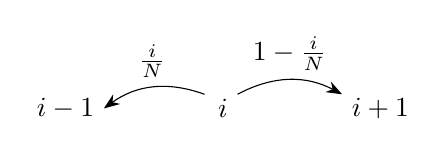
\begin{tikzpicture}[scale=1.0,>={Stealth[length=2mm]}]
  \node (a) at (0,0) {$i-1$};
  \node (b) at (2,0) {$i$};
  \node (c) at (4,0) {$i+1$};
  \draw[->] (b.west)+(0,0.18) ++(-0.05,0.18) to[bend right=28] node[above,pos=0.5]{$\frac{i}{N}$} (a.east);
  \draw[->] ($(b.east)+(0,0.18)$) to[bend left=28] node[above,pos=0.5]{$1-\frac{i}{N}$} ($(c.west)+(0,0.18)$);
\end{tikzpicture}
\end{center}
\end{example}

\begin{example}[$\lambda$-biased $\mathbb{T}^d$ SRW]
$\pi_i=C_{|i|}$（按层常数）。考虑 $A:=\{r:|r|\ge n\}$ 中之流动：
\[
\bigl(d^{\,n-1}\,C_{n-1}\bigr)\cdot\frac{d}{\lambda+d}
=\bigl(d^{\,n}\,C_n\bigr)\cdot\frac{\lambda}{\lambda+d}
\ \darr\quad
C_n=\frac1\lambda\,C_{n-1}
\ \darr\quad
C_n=\frac{1}{\lambda^n}\,C_0 .
\]
不变分布：$\sum_{i\in S}\pi_i=\sum_{n\ge0}d^{\,n}C_n=1\ \darr\
C_0=\Bigl(\sum_{n\ge0}\bigl(\tfrac d\lambda\bigr)^n\Bigr)^{-1}$。

结合 1.6.2 中结论有：
\[
\lambda\ge d\ \text{常返}\
\begin{cases}
\lambda>d\ \text{时正常返},\\
\lambda=d\ \text{时零常返};
\end{cases}
\qquad
\lambda<d\ \text{时非常返}.
\]
\end{example}

\begin{example}
设 $P$ 不可约、正常返，则
\[
\frac1n\sum_{m=0}^{n-1}\ind{X_m=i,\ X_{m+1}=j}\ \longrightarrow\ \pi_ip_{ij}
\quad\text{a.s.}
\]
\textbf{证法 1.} 令 $Y_n:=(X_n,X_{n+1})$，$\widetilde{S}:=\{(i,j):p_{ij}>0\}$，
$\widetilde{P}_{(i,j)(j,k)}=p_{jk}$，$\widetilde{\pi}_{(i,j)}=\pi_ip_{ij}$；
对 $\{Y_n\}$ 用遍历定理即可。

\textbf{证法 2.} 记 $r=V_i(n)$，则
\[
\frac1n\sum_{m=0}^{n-1}\ind{X_m=i,\ X_{m+1}=j}
=\frac{r}{n}\cdot\frac1r\sum_{s=0}^{r-1}\ind{X_{T_s+1}=j}
\xrightarrow{\ \text{LLN}\ }\pi_i\cdot p_{ij}
\quad\text{a.s.} \qed
\]
\end{example}

\secn{1.9}{强遍历定理}

\subsection*{1.9.1\quad 正常返、非周期}

$\dfrac1n\sum_{m=0}^{n-1}\Pp(X_m=i)\to\pi_i$。问：$\Pp(X_n=i)\to\pi_i$？（※）

\begin{example}[Ehrenfest，（※）的反例]
$S=\{0,1,\dots,N\}$，$\pi_i=\dbinom{N}{i}\dfrac{1}{2^N}$，$X_0=0$。则
$\Pp(X_{2n}=1)\equiv0,\ \forall n$。（周期性阻碍收敛。）
\end{example}

\begin{definition}[非周期]
若 $\exists\,N$，s.t.\ $\forall n>N$，$p_{ii}^{(n)}>0$，则称 $i$ \textbf{非周期}。
\end{definition}

\begin{proposition}
设 $P$ 不可约，存在非周期态，则任意状态非周期，且 $\exists\,N_{ij}$，s.t.\
$\forall n>N_{ij}$，$p_{ij}^{(n)}>0$。
\end{proposition}

\begin{proof}
设 $i$ 非周期。$\forall j\in S$，$\exists\,r_j,s_j$，s.t.\
$p_{ij}^{(r_j)}>0$，$p_{ji}^{(s_j)}>0$。取 $N_j=N_i+r_j+s_j$，则
\[
p_{jj}^{(n+r_j+s_j)}\ \ge\ p_{ji}^{(s_j)}\,p_{ii}^{(n)}\,p_{ij}^{(r_j)}>0,
\qquad \forall n\ge N_i .
\]
故 $j$ 非周期。同上述方法，$p_{ij}^{(n+r_j)}\ge p_{ii}^{(n)}p_{ij}^{(r_j)}>0\ (\forall n\ge N_i)$。 \qed
\end{proof}

\begin{theorem}[强遍历定理]
设 $P$ 不可约、正常返、非周期，则 $\forall\mu$：
\[
\sum_j\bigl|\Pp_\mu(X_n=j)-\pi_j\bigr|\ \longrightarrow\ 0 .
\]
\end{theorem}

\begin{proof}（耦合方法）

取 $\widetilde{S}:=S\times S$，$Z_n:=(W_n,Y_n)$，$r_{(i,j)(k,l)}:=p_{ik}\,p_{jl}$。

\textbf{1.}\ $Z_n$ 不可约、正常返：易知不变分布 $\widetilde{\pi}_{(i,j)}=\pi_i\times\pi_j$；
$Z_n$ 非周期：$r_{(i,j)(k,l)}^{(n)}=p_{ik}^{(n)}\,p_{jl}^{(n)}>0$（$n$ 充分大）。

\textbf{2.}\ $\tau:=\inf\{n\ge0:W_n=Y_n\}=\tau_D$，$D:=\{(i,i):i\in S\}$。则
$\tau\le\tau_{(i,i)}$，而 $\Pp(\tau_{(i,i)}<+\infty)=1$（常返），故
$\Pp(\tau<+\infty)=1$。

\textbf{3.}\ $\Pp(W_n=j,\ \tau\le n)=\Pp(Y_n=j,\ \tau\le n)$：事实上
\[
\text{LHS}=\sum_{m=0}^{n}\sum_{i\in S}\Pp(W_n=j,\ \tau=m,\ Z_m=(i,i))
=\sum_{m=0}^{n}\sum_{i\in S}\Pp(\tau=m,\ Z_m=(i,i))\cdot\Pp_{(i,i)}(W_{n-m}=j),
\]
而又由强马氏性有 $\Pp_{(i,i)}(W_{n-m}=j)=p_{ij}^{(n-m)}$。对 RHS 同理，故 LHS $=$ RHS。

\textbf{4.}\ 
\[
\bigl|\Pp(W_n=j)-\Pp(Y_n=j)\bigr|
=\bigl|\Pp(W_n=j,\tau\le n)-\Pp(Y_n=j,\tau\le n)
+\Pp(W_n=j,\tau>n)-\Pp(Y_n=j,\tau>n)\bigr|
\]
\[
\le\ \Pp(W_n=j,\tau>n)+\Pp(Y_n=j,\tau>n)\ \le\ 2\,\Pp(\tau>n),
\]
故 $\sum_j\bigl|\Pp(W_n=j)-\Pp(Y_n=j)\bigr|\le2\,\Pp(\tau>n)\to0$
（由 $\Pp(\tau<+\infty)=1$ 知 $\Pp(\tau>n)\to0$）。取 $\widetilde{S}$ 的初分布
$\nu=\mu\times\pi$ 即已得证。 \qed
\end{proof}

\end{document}
